% Curriculum  Vitae %
\documentclass[11pt]{article} %% Document parameters [<font_size>]
% Packages
%% Font
\usepackage[T1]{fontenc} %%% Font package
\usepackage{avant} %%% Font selection
\usepackage{array} %% Tables and arrays
\usepackage{babel} %% Multilingual typographic support
\usepackage{fontawesome5} %% Icons package %%% https://mirrors.ibiblio.org/CTAN/fonts/fontawesome5/doc/fontawesome5.pdf
\usepackage[a4paper,left=2cm, right=2cm, top=2cm, bottom=2cm]{geometry} %% Page structural settings
\usepackage{graphicx} %% Graphics and images
\usepackage{hyperref} %% Hyperlinks
\usepackage{makecell} %% Cells
\usepackage{enumitem} %% Enumerate / Itemize / Description
\usepackage{xcolor} %% Text color
\usepackage{pagecolor} %% Page color
\usepackage{framed} %% Text background box
\usepackage{fancyhdr} %% Header and footer text
\usepackage[utf8]{inputenc} %% Encoding
%\usepackage{showframe} %% Show page frame
% Variables
\def\firstname{Bastien} %% Firstname
\def\familyname{COLLOT} %% Name
\def\jobtitle{Data Analyst} %% Job title
\def\birthday{15 décembre 1994} %% Birth date 
\def\street{3 place du Sanitat} %% Street name
\def\city{44100 Nantes} %% City and county code
\def\email{collotbastien@gmail.com} %% Mail                    
\def\linkedin{linkedin.com/in/bastien-collot-210243153/} %% Likndin profile link
\def\phoneNumber{06 29 86 68 62} %% Phone number
\def\gitHubLink{github.com/bastien-data/cv/blob/master/BASTIEN_COLLOT_CV_READER.tex} %% LaTeX script GitHub link
%% Portrait
\graphicspath{ {./Images/} }
\def\portrait{
	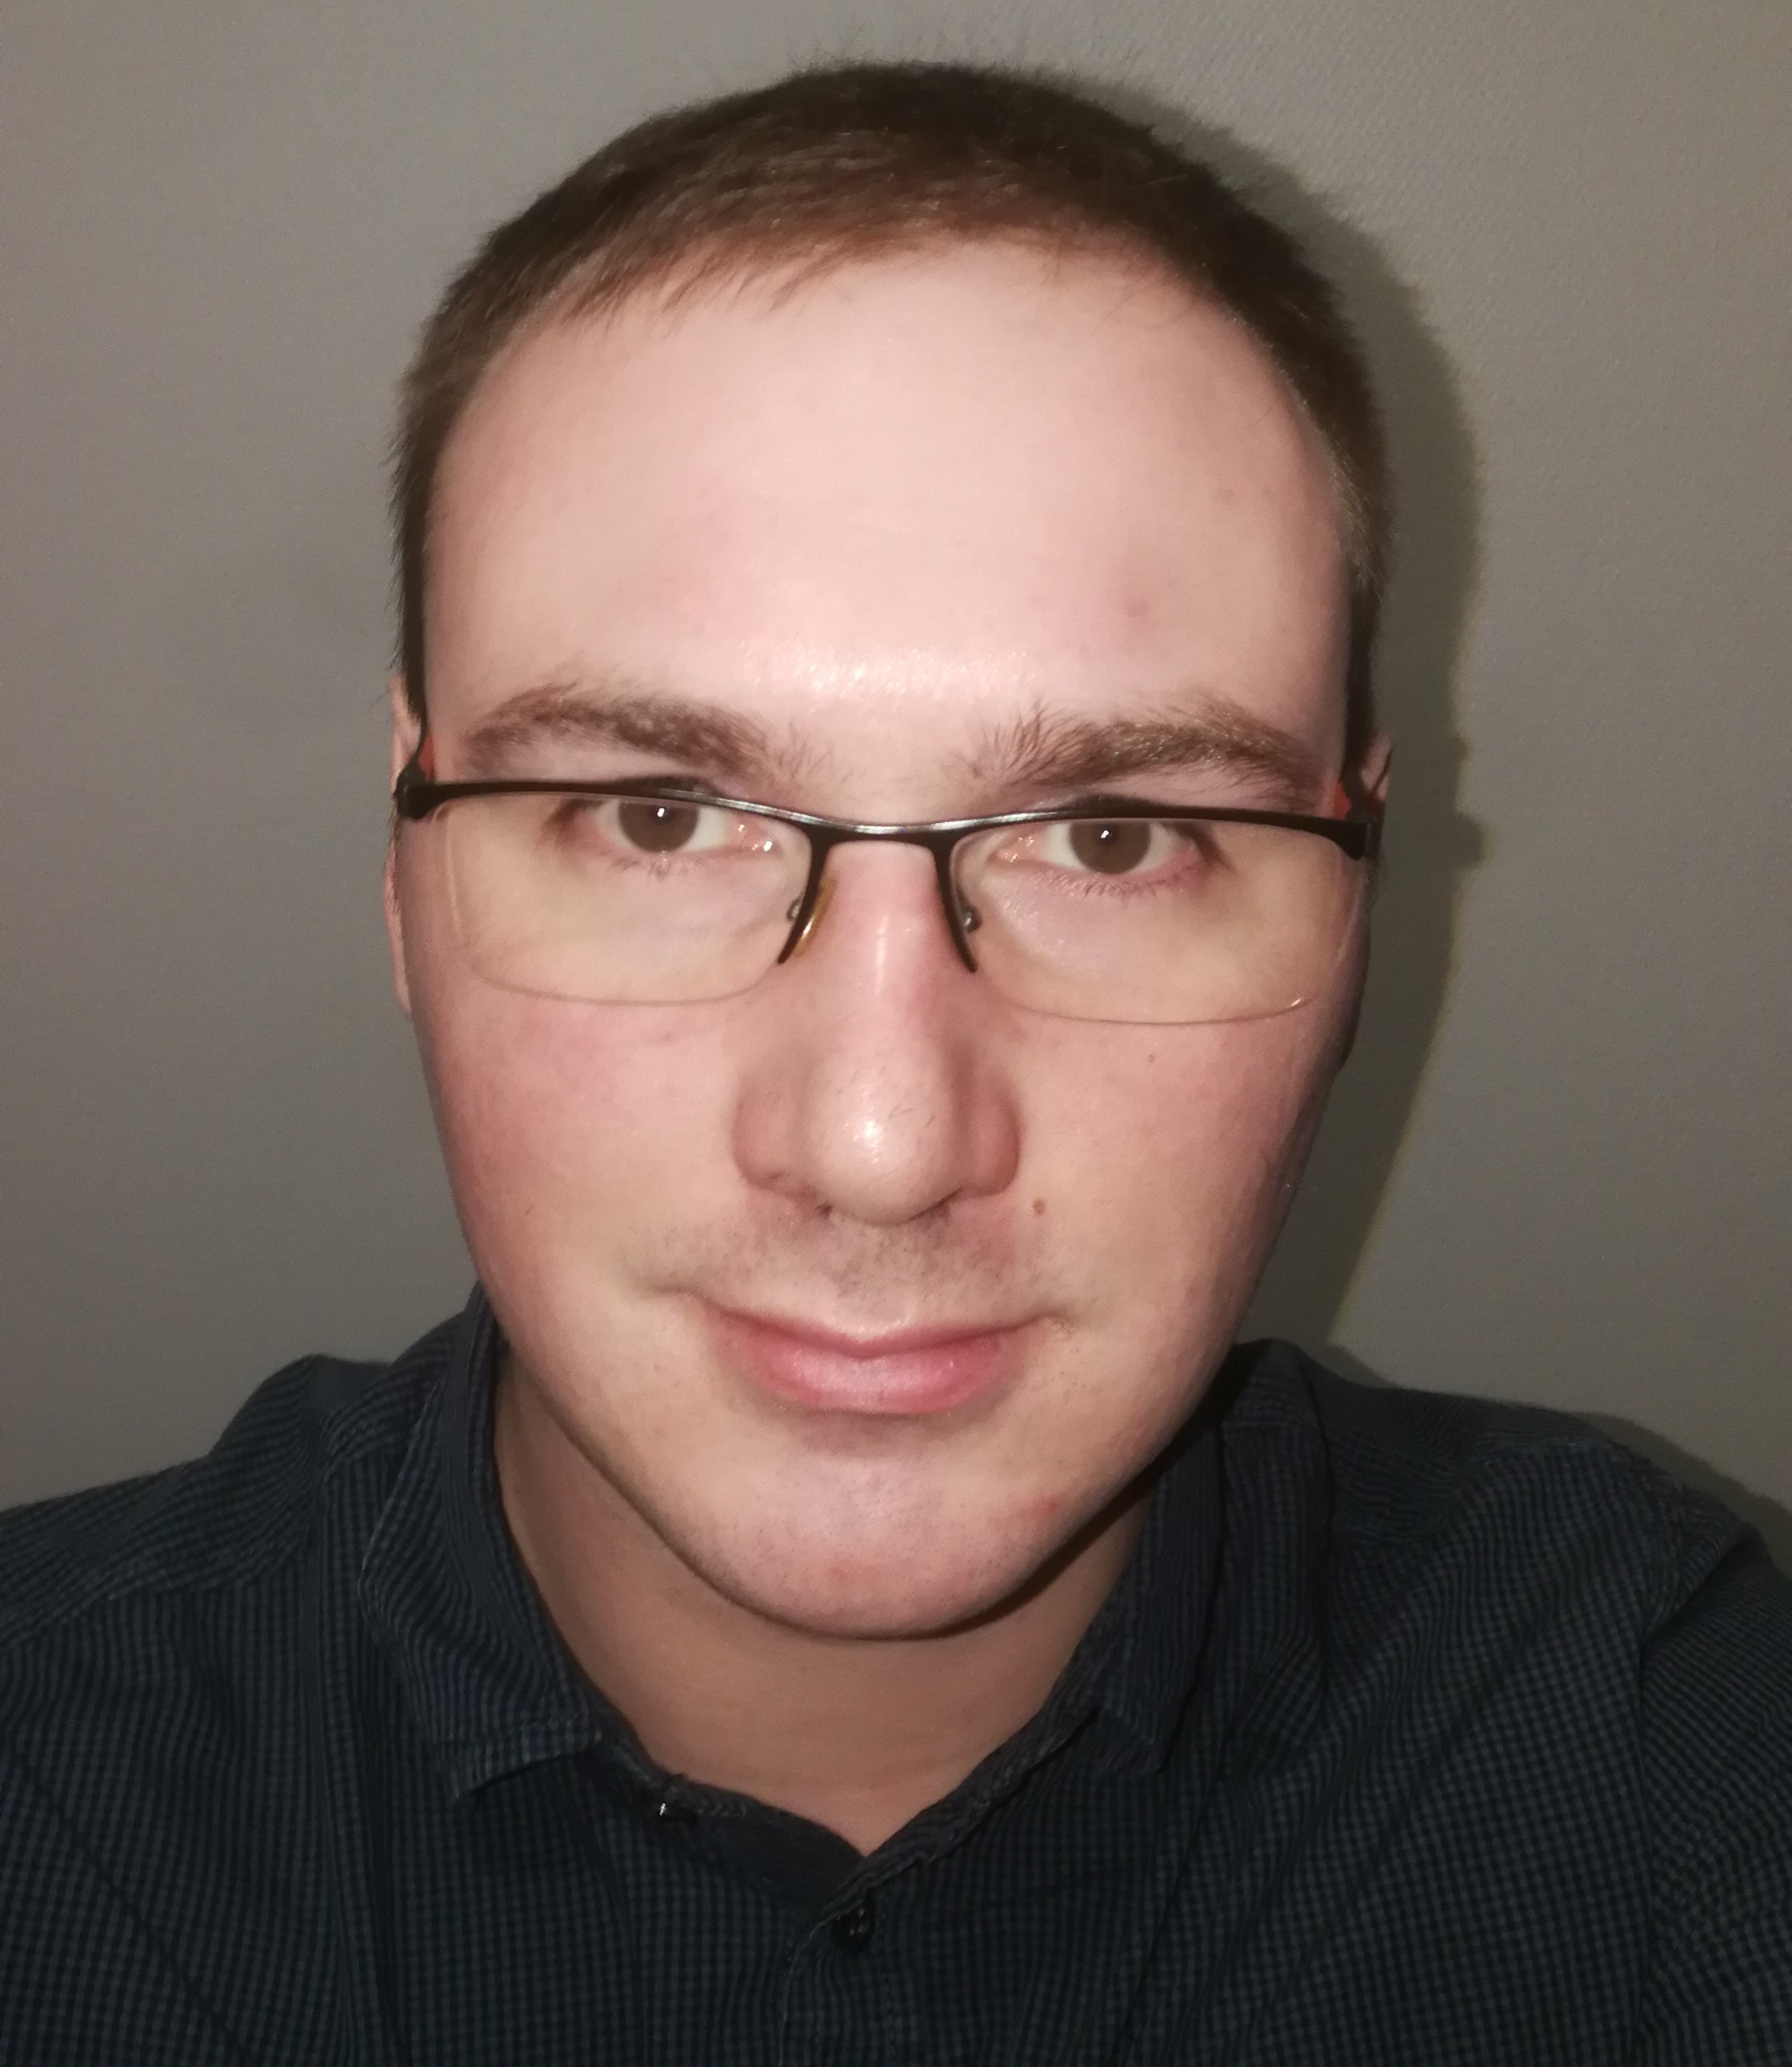
\includegraphics[scale=0.03]{
		{./Images/Portrait2.jpg}
	}
}
% Paramaters
%% fancyhdr
\pagestyle{fancy} %%% Set page style to fancy
\fancyhf{} %%% Clear header and footers
\renewcommand{\headrulewidth}{0pt} %%% Remove header line
\renewcommand{\familydefault}{\sfdefault} %% Set selected font as default
%% Hyperlink
\hypersetup{
	colorlinks=true,
	%%% Dark mode
	linkcolor=cyan,
	filecolor=cyan,      
	urlcolor=cyan,
	%%% White mode
	%linkcolor=blue,
	%filecolor=blue,      
	%urlcolor=blue,
	pdftitle={\firstname \familyname - \jobtitle},
	pdfauthor={\firstname \familyname}
}
%% Text, page and text background colors
%%% Dark mode
\pagecolor{black}
\color{white}
\definecolor{shadecolor}{RGB}{105,105,105} %%%% Dim grey
%%% White mode
%\pagecolor{white}
%\color{black}
%\definecolor{shadecolor}{RGB}{180,180,180} %%%% Grey
\pagenumbering{gobble} %% Disable page number
% Title definition
\renewcommand\maketitle{
	\par\noindent\begin{tabular}{ c c | c c }
		\makegapedcells
		\makecell[l]{
			\portrait
		} &
		\makecell[l]{
			\huge\firstname \\
			\huge\familyname
		} &
		\makecell[l]{
			\faPhone\ \phoneNumber \\ 
			\faEnvelope\ \href{mailto:\email}{\underline{\email}} \\
			\faBirthdayCake\ \birthday
		} &
		\makecell[l]{
			\faHome\ \street \\ \hspace{1.09em} \city \\
			\faLinkedinIn\ \href{https://www.\linkedin}{\firstname \: \familyname}
		}
	\end{tabular}
	\par\hrule
	\vspace{0.2cm}
	\centering\Large \textbf{\underline{Candidature de \Large\jobtitle}}
}
% Body
\begin{document}
	%% Generate title
	\maketitle
	\small
	%% Professional Experience
	\vspace{-1.2cm}
	\section*{\raggedright\large\textsc{\begin{snugshade*}Expérience professionnelle\end{snugshade*}}}
	\vspace{-0.5cm}
	\begin{description}
		\item \textbf{Mai 2024 - Oct 2024 | Consultant Data} chez \textbf{Keyrus}
		\begin{itemize}[noitemsep]
			\item Mission de data engineering pour le traitement et la centralisation de données.
			\begin{itemize}[noitemsep]
				\item Récolte des besoins métiers et rédaction des spéficiations techniques.
				\item Préparation, traitement et insertion des données par procédures Snowflake SQL.
				\item Implémentation de tests volumétriques et fonctionnelles.
				\item Gestion des versions, suivi des tickets et méthodologie agile. 
			\end{itemize}
		\end{itemize}
		\hrule
		\item \textbf{Sep 2022 - Mai 2024 | Développeur} chez \textbf{Armatis Business Consulting}
		\begin{itemize}[noitemsep]
			\item Modélisation, analyse et manipulation de bases de données PostgreSQL.
			\item Traitement et insertion de données  automatisés avec Talend.
			\item Calcul des indicateurs clés de performance et élaboration de rapports avec Power BI.
		\end{itemize} 
		\hrule
		\item \textbf{Sep 2021 - Sep 2022 | Alternant} chez \textbf{Armatis Business Consulting}
		\begin{itemize}[noitemsep]
			\item Formation pour le développement avec Power BI.
			\item Prototypage de rapports et tableaux de bords.
		\end{itemize} 
	\end{description}
	%% Skills
	\vspace{-1.5cm}
	\section*{\raggedright \large \textsc{\begin{snugshade*}Compétences\end{snugshade*}}}
	\vspace{-0.5cm}
	\begin{description}
		\item \textbf{Analyse et traitement de données structurées et semi-structurées}
		\par\begin{tabular}{l l l}
			• SQL et PL/SQL & • Snowflake & • PostgreSQL \\
			• Talend & • Data Analysis Expression (DAX) & • Excel / VisualBasic (VBA)
		\end{tabular}
		\hrule
		\item \textbf{Visualisation de données}
		\par\begin{tabular}{l l l}
			• Microsoft Power BI & • Tableau & • SAP BO Business Intelligence
		\end{tabular}
		\hrule
		\item \textbf{Modélisation de bases de données relationnelles}
		\par\begin{tabular}{l l l}
			• UML & • Modèle Entité / Association & • Méthodologie Merise
		\end{tabular}
		\hrule
		\item \textbf{Développement logiciel coopératif}
		\par\begin{tabular}{l l l l}
			• GitHub / GitLab & • Confluence & • Jira & • Méthodologie agile
		\end{tabular}
	\end{description}
	%% Soft skills
	\vspace{-1.5cm}
	\section*{\raggedright \large \begin{snugshade*}\textsc{Compétences secondaires}\end{snugshade*}}
	\vspace{-0.5cm}
	\begin{description}
		\item \textbf{Anglais}
		\par Niveau C1 (Certification TOEIC 2022).
		\hrule
		\item \textbf{Programmation}
		\par\begin{tabular}{l l l l}
			• Python & • Java & • Tests unitaires & • {\normalsize\fontfamily{cmr}\selectfont \LaTeX}
		\end{tabular}
	\end{description}
	%% Studies
	\vspace{-1.5cm}
	\section*{\raggedright \large \begin{snugshade*}\textsc{Etudes}\end{snugshade*}}
	\vspace{-0.5cm}
	\begin{description}
		\item \textbf{2021 - 2022 | Licence Professionelle Big Data (\,LP BDB)\,} 
		\par\hspace{1.45cm} Université de Bordeaux à l'IUT de Périgeux
		\item \textbf{2018 - 2020 | DUT Statistique et Informatique Décisionnelle (\,DUT STID)\,} 
		\par\hspace{1.45cm} Université de Poitiers à l'IUT de Niort
		\item \textbf{2015 - 2017 | Bachelor Game Design} 
		\par\hspace{1.45cm} École Bellecour à Lyon
		\item \textbf{2013 - 2014 | L1 de Gestion et Communication} 
		\par\hspace{1.45cm} Institut des Stratégies et Techniques de Communication (ISTC) à Lille
		\item \textbf{2012 - 2013 | L1 d'Économie et Gestion} 
		\par\hspace{1.45cm} Faculté Libre de Sciences Economiques et de Gestion (FLSEG) à Lille
	\end{description}
	\fancyfoot[C]{\faGithub \href{https://www.\gitHubLink}{ \, \underline{GitHub}}}
\end{document}

